\section{光线追踪}
\subsection{路径追踪基本}
要利用路径跟踪算法,实现一个全局光照模型,至少需要解决四方面的问题:
\begin{enumerate}
\item 场景、物体、材料的数据结构,物体数据结构中需要存储坐标和一些必要的属性缓存信息,如法向量。材料的数据结构中主要存储材料的参数。
\item 实现光线与场景的交互,包括计算交点、折射、反射、漫反射。
\item 实现颜色模型,即处理颜色如何叠加。
\item 输出可视化结果。
\end{enumerate}

对于第一个问题,本文使用三角面片来表示物体,每个物体用一个基类表示,所有物体继承这个基类,内部存储三角面片的坐标、面法向量、顶点法向量。由于是光线追踪类模型是从屏幕的像素点发射光线到场景中,因此主要问题是把屏幕“放置”到世界中,确实3D坐标。不必考虑怎么将3D坐标投影到屏幕的2D坐标。

本文采用的方式是将屏幕放在XY平面,屏幕中心就是原点。如下图所示:

\begin{center}
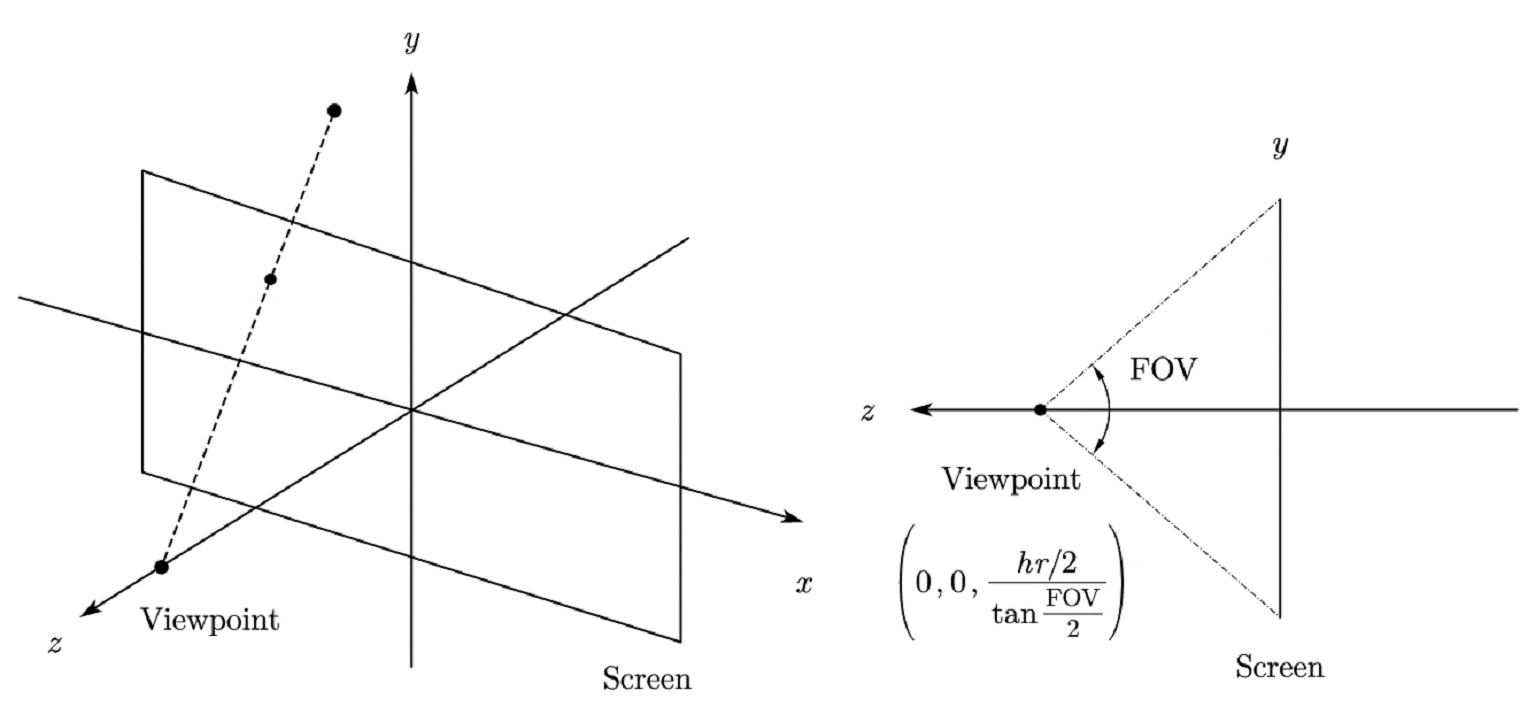
\includegraphics[width=10cm]{figure/screen.png}
\end{center}

对于第二个问题。路径追踪的思路是从每个像素点射出若干条射线,射线如果遇到三角面片,会以一定概率发生反射、折射、漫反射,这由材料的属性决定,最终假如遇到了光源,就可以计算像素的颜色了。示意图如下:

\begin{center}
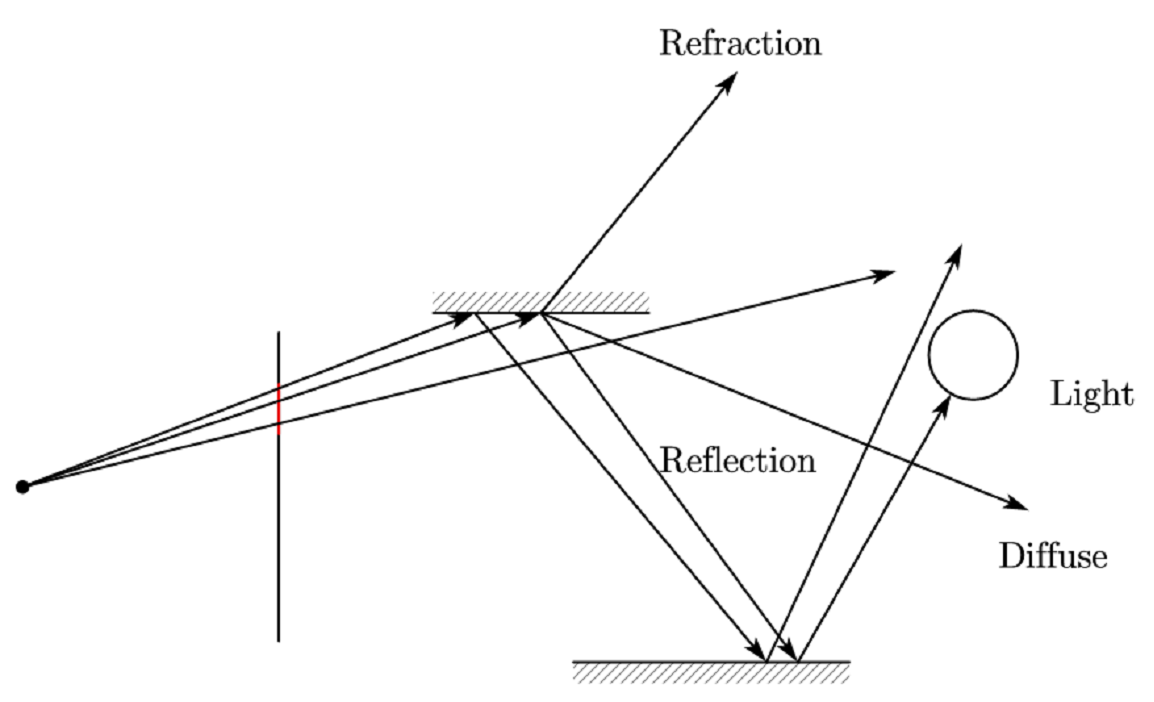
\includegraphics[width=10cm]{figure/path tracing.png}
\end{center}

一个首要的问题就是计算射线与三角面片的交点。本文使用了NanoRT库,它就是用来计算交点。使用这个库是因为它使用了加速算法,如果自己实现一遍,手动遍历所有面片来计算交点,则效率会很低。

在计算交点以后,需要计算折射、反射与漫反射的概率。按下式给出:

\begin{center}
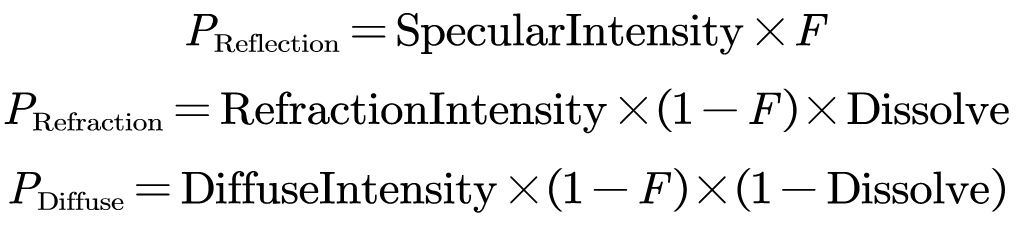
\includegraphics[width=6cm]{figure/prob.png}
\captionof{figure}{反射、折射、漫反射概率}
\label{prob}
\end{center}
基中$F$值为Fresnel效应值,按下式逼近:
\begin{center}
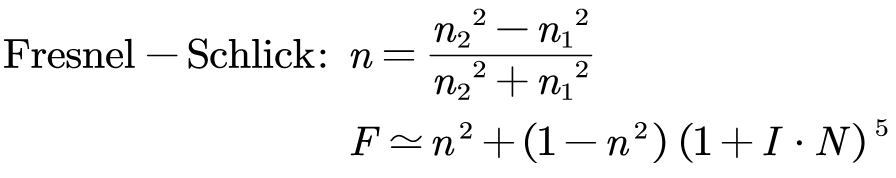
\includegraphics[width=6cm]{figure/fresnel.png}
\end{center}
$I,N$分别为入射光线的方向向量、法向量,参考后面的折射公式。当入射光线接近垂直于平面时,$I\cdot N$会接近0,于是折射效应强烈。注意以上三个值的和并不为1,需要归一化后才能用来进行采样。

然后需要计算每种情形下的光线。前两个的示意图如下:

\begin{center}
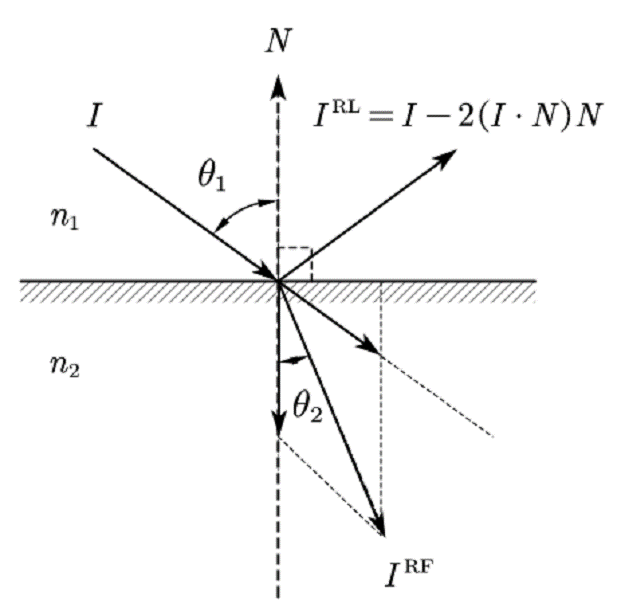
\includegraphics[width=6cm]{figure/reflection and refraction.png}
\end{center}

反射可以直接通过几何计算出来,而折射需要考虑物理效应:Fresnel效应,计算公式如下:

\begin{center}
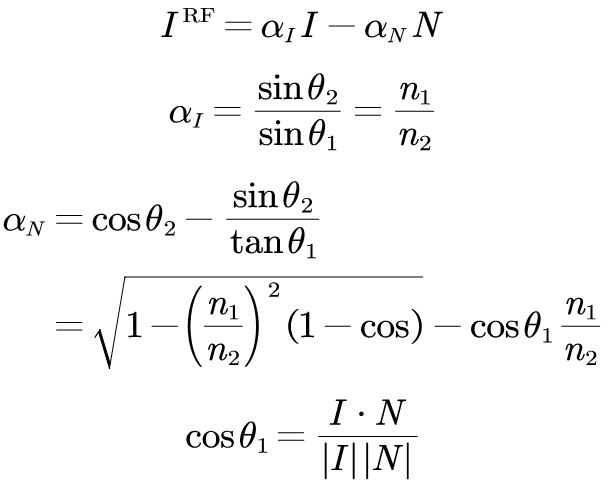
\includegraphics[width=6cm]{figure/refraction formula.png}
\end{center}

在计算漫反射时,首先建立一个局部坐标系,随机从坐标在原点的上半球上采样一点作为漫反射的采样光线,再把这条光线进行旋转、平移,使原点变换为入射光线与面片的交点,使$z$轴与面片的法向相同,公式如下:

\begin{center}
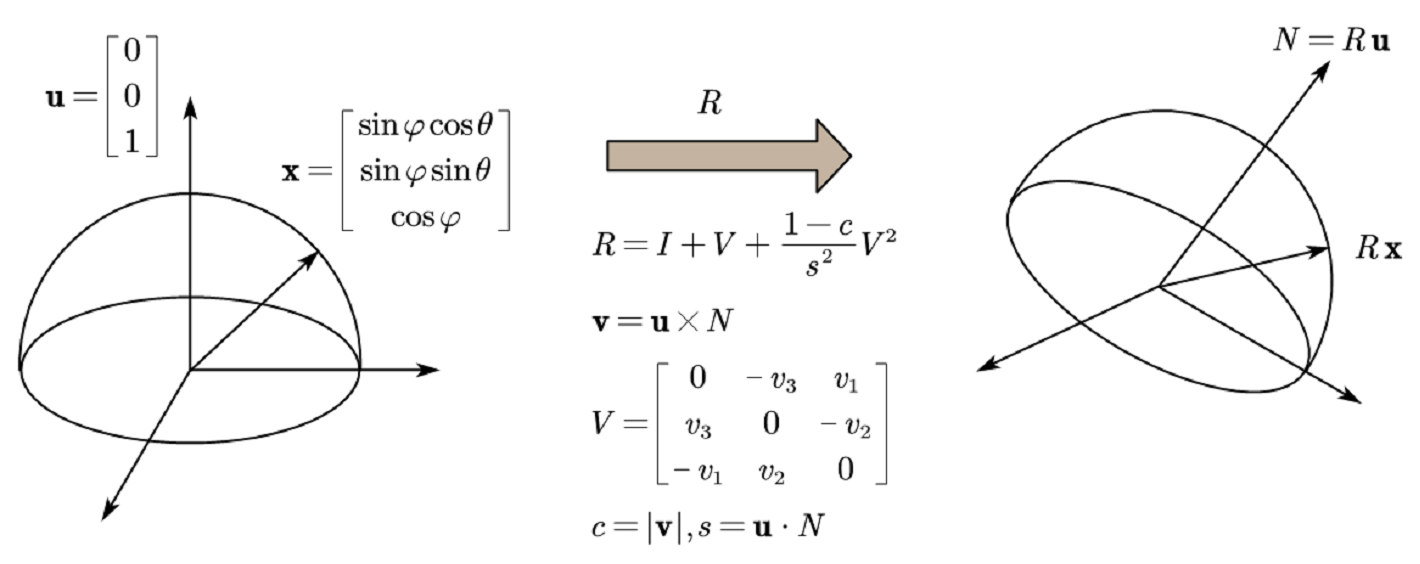
\includegraphics[width=12cm]{figure/diffuse.png}
\end{center}

然后需要确定颜色模型,即如何确定每条光线给像素的着色。本文对每条光线首先赋予一个3D向量$w=[1,1,1]^T$作为权重。此后,按以下方式在光线发生折射、反射、漫反射时更新权重:
\begin{enumerate}\label{color-model}
\item 反射:$w'=w\odot specular$
\item 漫反射:$w'=w\odot diffuse$
\item 折射:$w'=w\odot transmittance$
\item 光源:$c=w\cdot emission$
\end{enumerate}
其中$\odot$为element-wise乘法,specular、diffuse、transmittance、emission为材料的参数,$c$为最终的像素颜色。
